\documentclass[12pt,a4paper]{article}

% load packages
\usepackage{xcolor}
\usepackage{graphicx}
\usepackage{amsmath}
\usepackage{amsfonts}
\usepackage{amssymb}
\usepackage{parskip}
\usepackage{tikz}
\usepackage{listings}
\usepackage{hyperref}
\usepackage{algorithm}
\usepackage{algpseudocode}
\usepackage[left=2cm,right=2cm,top=2cm,bottom=2cm]{geometry}

% set code style
\definecolor{codegreen}{rgb}{0,0.6,0}
\definecolor{codegray}{rgb}{0.5,0.5,0.5}
\definecolor{codepurple}{rgb}{0.58,0,0.82}
\definecolor{backcolour}{rgb}{0.95,0.95,0.92}

% set lst style
\lstdefinestyle{mystyle}{
    backgroundcolor=\color{backcolour},   % 设置背景颜色
    commentstyle=\color{codegreen},
    keywordstyle=\color{magenta},
    numberstyle=\tiny\color{codegray},
    stringstyle=\color{codepurple},
    basicstyle=\ttfamily\footnotesize,    % 使用等宽字体
    breakatwhitespace=false,         
    breaklines=true,                 
    captionpos=b,                    
    keepspaces=true,                 
    numbers=left,                    
    numbersep=5pt,                  
    showspaces=false,                
    showstringspaces=false,
    showtabs=false,                  
    tabsize=2
}
\lstset{style=mystyle}


\title{Project 2 Report for Probelm 2.1}
\author{Zhu Liang}
\date{\today}

\begin{document}

\maketitle

\section{Project Description}
In this project, we undertake two primary tasks. 
The first task is to provide a detailed description of the algorithms behind five collective communication operations provided by MPI.
The description are provided in Section \ref{sec:mpi_buildin}.
The second task is an empirical comparison between the built-in \texttt{MPI\_Bcast} and a custom broadcast implementation named \texttt{MY\_Bcast()}.


\section{Algorithm Description}
\subsection{MPI Build-in Operations}
\label{sec:mpi_buildin}


\textbf{\texttt{MPI\_Bcast()}}: This function broadcasts a message from the process with the designated root rank to all other processes in the communicator. All processes must call this function, with matching arguments.

\textbf{\texttt{MPI\_Scatter()}}: This function distributes distinct blocks of data from the root process to each process in the communicator. The root sends data to itself as well as to the other processes.

\textbf{\texttt{MPI\_Allgather()}}: Each process sends its own data to all other processes and gathers data from all processes. At the end, every process has the data from all the other processes.

\textbf{\texttt{MPI\_Alltoall()}}: This function allows each process to send distinct data to every other process. It generalizes the functionality of both scatter and gather, with different data being sent to each process.

\textbf{\texttt{MPI\_Reduce()}}: All processes in the communicator contribute their own data, which is combined (reduced) into a single result using a specified operation, like sum, max, etc. The result is stored on the root process.


\subsection{Custom Broadcast Function: \texttt{MY\_Bcast()}}
In large-scale parallel computations, efficient data transfer across processes is paramount. 
A simple broadcast approaches, 
which involve a root process sending messages to every other process sequentially, 
can be inefficient, 
especially when the number of processes grows, 
leading to a linear time complexity of $O(n)$.

To enhance this, 
we leverage it with a binary tree structure. 
Here, each process communicates only with its parent and potential left and right children (when children exist). 
Thus, it works even when the number of processes is not a power of 2.
The root initiates the broadcast, and the message cascades down the tree, reaching all processes.
Pleasee refer to Figure \ref{fig:binary_tree} for an illustration of the binary tree structure when $P = 4$.
This approach reduces the time complexity from $O(n)$ to $O(log(n))$.

For more details on the project structure and the implementation, 
please refer to the \texttt{README.md} file in the \texttt{project2} folder.

The pseudocode is shown below.
\begin{algorithm}
    \caption{Custom Broadcast Function Using Binary Tree}
    \begin{algorithmic}[1]
    \Procedure{MY\_ Bcast}{}
    \State \textbf{Get} rank and size of processes
        \If{current process rank is not \textit{root}}
            \State \textbf{Receive} content of buffer from \textit{parent} 
        \EndIf
        \If{left child exists}
            \State \textbf{Send} content of buffer to \textit{left child} 
        \EndIf
        \If{right child exists}
            \State \textbf{Send} content of buffer to \textit{right child} 
        \EndIf
        \State \Return MPI\_SUCCESS
    \EndProcedure
    \end{algorithmic}
\end{algorithm}
\begin{figure}
    \centering
    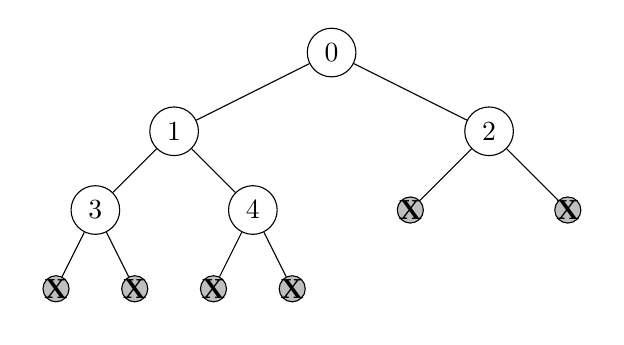
\begin{tikzpicture}[
        every node/.style = {circle, draw},
        missing/.style={fill=gray!50, label=center:{\textbf{X}}},
        level distance = 10mm,
        level 1/.style = {sibling distance=40mm},
        level 2/.style = {sibling distance=20mm},
        level 3/.style = {sibling distance=10mm},
      ]
      
      \node {0}
        child {node {1}
          child {node {3}
            child {node[missing] {}}
            child {node[missing] {}}
          }
          child {node {4}
            child {node[missing] {}}
            child {node[missing] {}}
          }
        }
        child {node {2}
          child {node[missing] {}}
          child {node[missing] {}}};
      
    \end{tikzpicture}
    \caption{Binary Tree Structure when $P = 4$}
    \label{fig:binary_tree}
\end{figure}


  
  
  
  
\section{Results}

In the following tables, 
we present the execution times for two different broadcast implementations: 
\texttt{MPI\_Bcast} and \texttt{MY\_Bcast}. 
It is essential to note that while individual run times might vary depending on the specific runtime environment, 
the general pattern observed should remain similar across different runs.

\begin{table}[!htb]
    \centering
    \begin{tabular}{|c|c|c|c|c|}
    \hline
    & P = 4 & P = 7 & P = 28 & P = 37 \\
    \hline
    $N = 2^{10}$ & 0.000010s & 0.000059s & 0.000045s & 0.000069s \\
    \hline
    $N = 2^{12}$ & 0.000023s & 0.000054s & 0.000061s & 0.000063s \\
    \hline
    $N = 2^{14}$ & 0.000036s & 0.000057s & 0.000151s & 0.000181s \\
    \hline
    $N = 2^{16}$ & 0.000120s & 0.000125s & 0.000454s & 0.000526s \\
    \hline
    \end{tabular}
    \caption{Execution time using \texttt{MPI\_Bcast}}
    \end{table}

\begin{table}[!htb]
    \centering
    \begin{tabular}{|c|c|c|c|c|}
    \hline
    & P = 4 & P = 7 & P = 28 & P = 37 \\
    \hline
    $N = 2^{10}$ & 0.000012s & 0.000020s & 0.000057s & 0.000086s \\
    \hline
    $N = 2^{12}$ & 0.000010s & 0.000024s & 0.000072s & 0.000091s \\
    \hline
    $N = 2^{14}$ & 0.000021s & 0.000058s & 0.000123s & 0.000145s \\
    \hline
    $N = 2^{16}$ & 0.000057s & 0.000165s & 0.000385s & 0.000416s \\
    \hline
    \end{tabular}
    \caption{Execution time using \texttt{MY\_Bcast}}
    \end{table}

\section{Analysis}

Based on the empirical results obtained, 
both \texttt{MPI\_Bcast()} and our custom implementation \texttt{MY\_Bcast()} demonstrate closely matched performance. 
This is a significant observation given that the \texttt{MY\_Bcast()} function was optimized to operate in \(O(\log(n))\) time complexity, 
using a binary tree approach.

\section*{File Notes}
The source code of the program is in the \texttt{project2} folder. 
For more details, please refer to the \texttt{README.md} file in the folder.

\end{document}
